\documentclass[11pt,a4paper]{article}

\usepackage[utf8]{inputenc}
\usepackage[T1]{fontenc}
\usepackage[expansion=false]{microtype}
\usepackage[margin=1in]{geometry}
\usepackage{amsmath,amssymb,amsfonts,amsthm,mathtools}
\usepackage{bm}
\usepackage{booktabs}
\usepackage{multirow}
\usepackage{array}
\usepackage{xcolor}
\usepackage{tikz}
\usetikzlibrary{arrows.meta,positioning,shapes.geometric,calc,fit}
\usepackage[colorlinks=true,linkcolor=blue!70!black,citecolor=teal!70!black,urlcolor=blue!70!black]{hyperref}

\newtheorem{theorem}{Theorem}[section]
\newtheorem{proposition}[theorem]{Proposition}
\newtheorem{lemma}[theorem]{Lemma}
\newtheorem{corollary}[theorem]{Corollary}
\theoremstyle{definition}
\newtheorem{definition}[theorem]{Definition}
\theoremstyle{remark}
\newtheorem{remark}[theorem]{Remark}

\newcommand{\R}{\mathbb{R}}
\newcommand{\C}{\mathbb{C}}
\newcommand{\Ha}{\mathbb{H}}
\newcommand{\Oc}{\mathbb{O}}
\newcommand{\Se}{\mathbb{S}}
\newcommand{\Ftwo}{\mathbb{F}_2}
\newcommand{\PG}{\mathrm{PG}}
\newcommand{\ImPart}{\mathrm{Im}}
\newcommand{\RePart}{\mathrm{Re}}
\newcommand{\Falt}{\mathcal{F}_{\mathrm{alt}}}
\newcommand{\Fzd}{\mathcal{F}_{\mathrm{ZD}}}
\newcommand{\PiMoreno}{\Pi_{\mathrm{Moreno}}}
\newcommand{\PiNull}{\Pi_{\ker L}}
\newcommand{\popcount}{\mathrm{popcount}}

\title{\textbf{Sedenion $\PG(3,2)$ Zero-Divisor Beamforming for GNSS\\
Anti-Jamming and Anti-Spoofing: Matrix-Inversion-Free Null Steering,\\
Associative Quaternion Phase Hinges, and Neural CRPA Validation}}

\author{
  \textbf{Dionisio Chiuratto Agourakis}\thanks{Correspondence: \href{mailto:dionisio.ca@gmail.com}{\texttt{dionisio.ca@gmail.com}}. Official archival preprint and benchmark suite registered at Zenodo DOI \href{https://doi.org/10.5281/zenodo.23603006}{\texttt{10.5281/zenodo.23603006}}; companion algebraic foundations and Lean~4 formalization archived at Zenodo DOI \href{https://doi.org/10.5281/zenodo.23588274}{\texttt{10.5281/zenodo.23588274}} (\url{https://github.com/josaum/sedenion-pg32}).} \\[0.4em]
  \small \href{mailto:dionisio.ca@gmail.com}{\texttt{dionisio.ca@gmail.com}} $\;\cdot\;$ \href{https://doi.org/10.5281/zenodo.23603006}{\texttt{doi:10.5281/zenodo.23603006}}
}

\date{October 2026}

\begin{document}

\maketitle

\begin{abstract}
\noindent
Global Navigation Satellite System (GNSS) signals such as GPS L1 C/A arrive at terrestrial receivers roughly $20\,\mathrm{dB}$ below the thermal noise floor ($\approx -130\,\mathrm{dBm}$), making them vulnerable to high-power wideband barrage jammers, swept-frequency chirp interferers, and repeater/meaconing spoofers operating at $+60\text{ to }+80\,\mathrm{dB}$ Jammer-to-Signal Ratio ($\mathrm{JSR}$). Classical Space-Time Adaptive Processing (STAP) and Minimum Variance Distortionless Response (MVDR / Capon) beamformers on 8-element Controlled Reception Pattern Antennas (CRPAs) require $\mathcal{O}(d^3)$ sample covariance matrix inversions ($\hat{\bm{R}}_{xx}^{-1}$) that become ill-conditioned at extreme $\mathrm{JSR}$, suffer from finite-sample sidelobe bleed under non-stationary jammer drift, and induce carrier-phase discontinuities (Phase-Locked Loop cycle slips) when switching spatial nulls. Conversely, hypercomplex polarimetric array processors based on normed division algebras---complex ($\C^8$), quaternion ($\Ha^4$), and octonion ($\Oc^2$) arrays---are algebraically prohibited by Hurwitz's theorem ($\|u \cdot v\|_2 = \|u\|_2 \|v\|_2$) from nulling an interferer via single-channel multiplication.

In this paper, we map the 16 real baseband degrees of freedom of an 8-element complex CRPA ($\C^8 \cong \R^{16}$) directly onto the 16-dimensional Cayley--Dickson \textbf{sedenion algebra} ($\Se = \Oc \oplus \Oc e_8$) governed by the finite projective 3-space $\PG(3,2)$ \cite{Agourakis2026PG32}. We establish three results for electronic warfare (EW) and navigation integrity:
\begin{enumerate}
    \item \textbf{Matrix-Inversion-Free $\mathcal{O}(1)$ Jammer Annihilation:} Projecting the dominant jammer spatial-polarimetric signature onto the 11-dimensional Moreno--Stiefel cone $u_{\mathrm{jam}} = (a, b) \in V_2(\R^7) \subset \Se$ yields a closed-form 4-dimensional nullspace operator $v_{\mathrm{beam}} = \PiNull(u_{\mathrm{jam}}; c_{\mathrm{sat}}) = (c_{\mathrm{sat}}, (a \cdot_{\Oc} c_{\mathrm{sat}}) \cdot_{\Oc} b) \in \ker L_{\Se}(u_{\mathrm{jam}})$ that annihilates the jammer identically ($u_{\mathrm{jam}} \cdot_{\Se} v_{\mathrm{beam}} = 0$) in $\mathcal{O}(1)$ operations without covariance inversion, achieving $\mathbf{139.1\,\mathrm{dB}}$ jammer suppression in FP32 ($\mathbf{312.9\,\mathrm{dB}}$ in FP64) and $\mathbf{100.0\%}$ GPS L1 C/A 1023-chip Gold-code acquisition at $\mathrm{JSR} = +80\,\mathrm{dB}$ (where MVDR-SMI, Softmax, $\Ha^4$, $\Oc^2$, and $\mathcal{Cl}_{0,4}$ fail).
    \item \textbf{Cycle-Slip-Free RTK Carrier-Phase Tracking via $\PG(3,2)$ Quaternion Hinges:} Using the $8+7$ Fano hyperplane bifurcation of $\PG(3,2)$, the receiver routes benign tracking through the 8 norm-preserving octonion workspaces ($\Falt \cong \Oc$) and jammer excision through the 7 quasi-octonion zero-divisor workspaces ($\Fzd \cong \tilde{\Oc}$). Because any workspace pair $(H_{\omega_1}, H_{\omega_2})$ intersects in a 3-node associative quaternion hinge $L_{12} = H_{\omega_1} \cap H_{\omega_2} \cong \Ha$, quadrature $(e_i, e_j)$ carrier phase is preserved with $\mathbf{0.0000^\circ}$ phase jump error and $\mathbf{0.0\%}$ PLL cycle-slip rate during dynamic null switches.
    \item \textbf{Multi-Spoofer Neural CRPA Rejection:} Using Orthogonal Half-Sphere Key Modulation, our parameter-matched \texttt{Sed-PG32-Moreno} and \texttt{Sed-PG32-Moreno-NoFFN} ($-47.4\%$ parameters) neural CRPA receivers achieve $\mathbf{100.0\%}$ in-distribution and out-of-distribution navigation integrity accuracy with $\mathbf{0.0\%}$ Spoofer False-Lock Rate (FLR).
\end{enumerate}
\end{abstract}

\noindent\textbf{Keywords:} GPS Anti-Jamming, GNSS Anti-Spoofing, Controlled Reception Pattern Antenna (CRPA), Space-Time Adaptive Processing (STAP), Sedenion Zero Divisors, Finite Projective Space $\PG(3,2)$, Moreno Cone, Carrier Phase Tracking.

\vspace{1em}
\hrule
\vspace{1.5em}

% ==============================================================================
% SECTION 1: INTRODUCTION
% ==============================================================================
\section{Introduction}
\label{sec:intro}

Civilian and military Global Navigation Satellite Systems (GNSS) rely on Direct-Sequence Spread Spectrum (DSSS) pseudorandom noise (PRN) codes---such as the 1023-chip Gold codes of GPS L1 C/A at $1575.42\,\mathrm{MHz}$ \cite{ISGPS200,Kaplan2017}---to recover satellite signals arriving at $-125\text{ to }-135\,\mathrm{dBm}$, approximately $20\,\mathrm{dB}$ below ambient thermal noise in a $2\,\mathrm{MHz}$ bandwidth. While the $10\log_{10}(1023) \approx 30.1\,\mathrm{dB}$ spreading gain enables reliable acquisition under benign thermal noise ($\mathrm{SNR}_{\mathrm{pre}} = -20\,\mathrm{dB} \to \mathrm{SNR}_{\mathrm{post}} \approx +10.1\,\mathrm{dB}$), intentional Radio Frequency Interference (RFI) easily overwhelms this margin \cite{BorIO2018,Amin2016}. A $1\,\mathrm{W}$ portable jammer at $5\,\mathrm{km}$ produces a Jammer-to-Signal Ratio ($\mathrm{JSR}$) of $+60\text{ to }+80\,\mathrm{dB}$, raising the post-correlation interference floor $30\text{ to }50\,\mathrm{dB}$ above the GPS correlation peak. Simultaneously, repeater (meaconing) and coherent GNSS spoofers \cite{Psiaki2016} broadcast delayed or synthesized PRN replicas that capture the receiver's Delay-Locked Loop (DLL) and Phase-Locked Loop (PLL), inducing hazardous navigation false locks.

Multi-antenna Controlled Reception Pattern Antennas (CRPAs) and Space-Time Adaptive Processing (STAP) mitigate spatial interference by forming adaptive nulls toward jammer directions of arrival (DOAs) \cite{VanTrees2002,Compton1988}. However, existing algebraic and neural beamforming paradigms face three fundamental structural limitations:
\begin{enumerate}
    \item \textbf{Ill-Conditioned $\mathcal{O}(d^3)$ Covariance Inversion and Finite-Sample Sidelobe Bleed:} Classical Minimum Variance Distortionless Response (MVDR / Capon) Sample Matrix Inversion (SMI) estimates the $d \times d$ covariance matrix $\hat{\bm{R}}_{xx} = \frac{1}{K}\sum_{k=1}^K \bm{x}_k \bm{x}_k^{\mathrm{H}} + \delta \bm{I}$ and computes $\bm{w}_{\mathrm{MVDR}} \propto \hat{\bm{R}}_{xx}^{-1}\bm{a}(\theta_{\mathrm{sat}})$. At $\mathrm{JSR} = +80\,\mathrm{dB}$ ($\mathrm{JNR} = +60\,\mathrm{dB}$), the condition number $\kappa(\hat{\bm{R}}_{xx}) \ge 10^6$ amplifies FP32 numerical round-off, while diagonal loading $\delta$ and sub-degree jammer DOA drift limit practical null depth to $40\text{--}50\,\mathrm{dB}$, leaking $+10\text{ to }+20\,\mathrm{dB}$ of residual jammer power into the PRN correlator. Similarly, neural softmax attention beamformers assign strictly positive weights ($\alpha_j = \exp(z_j)/\sum_k \exp(z_k) > 0$), suffering from probabilistic ``softmax bleed'' that cannot hard-zero a $+80\,\mathrm{dB}$ jammer.
    \item \textbf{The Hurwitz Division-Algebra Obstruction in Polarimetric Arrays:} Complex ($\C$), quaternion ($\Ha$) \cite{Bihan2004}, and octonion ($\Oc$) signal processors preserve Euclidean norms under multiplication: $\|u \cdot v\|_2 = \|u\|_2 \|v\|_2$. Consequently, no non-zero hypercomplex filter weight $v \neq 0$ can annihilate a non-zero jammer state $u \neq 0$ ($u \cdot v = 0$) within a single algebraic channel.
    \item \textbf{Carrier-Phase Discontinuities (PLL Cycle Slips) Under Null Switching:} In high-precision Real-Time Kinematic (RTK) and carrier-phase navigation, re-computing unconstrained MVDR weights when a jammer activates or changes azimuth rotates the complex phase of the satellite passband response, triggering PLL cycle slips ($\Delta\phi > 15^\circ$).
\end{enumerate}

In this work, building directly on the algebraic and Lean~4 machine-checked framework of \cite{Agourakis2026PG32}, we show that an 8-element complex CRPA (or a 4-element dual-polarized RHCP/LHCP array with 2 delay taps), possessing $2 \times 8 = 16$ real baseband degrees of freedom, maps isomorphically onto the 16-dimensional \textbf{sedenion algebra} $\Se = \Oc \oplus \Oc e_8$. Rather than treating sedenion zero divisors and non-associativity as algebraic pathologies, we exploit them to construct an $\mathcal{O}(1)$ matrix-inversion-free null-steering beamformer, a cycle-slip-free $\PG(3,2)$ quaternion hinge router, and a multi-spoofer neural CRPA architecture.

% ==============================================================================
% SECTION 2: 16D SEDENION BASEBAND CRPA MODEL & MORENO NULL STEERING
% ==============================================================================
\section{16D Sedenion Baseband CRPA Model and $\mathcal{O}(1)$ Moreno Null Steering}
\label{sec:crpa_model}

\subsection{Isomorphism Between an 8-Element Complex CRPA and $\Se$}
Consider an 8-element GNSS CRPA (or a 4-element dual-polarized RHCP/LHCP array with 2 temporal taps) sampling the L1 C/A baseband signal at chip rate $R_c = 1.023\,\mathrm{MHz}$. At chip index $t \in \{0, \dots, L-1\}$ ($L = 1023$), the 8 complex in-phase and quadrature ($I/Q$) antenna outputs $\bm{z}(t) = [I_0(t) + \mathrm{i}Q_0(t), \dots, I_7(t) + \mathrm{i}Q_7(t)]^\top \in \C^8$ assemble into a 16-dimensional real sedenion vector $X(t) \in \Se \cong \R^{16}$:
\begin{equation}
\label{eq:sedenion_snap}
X(t) = \sum_{m=0}^{7} \Big( I_m(t) \, e_m + Q_m(t) \, e_{m+8} \Big) = \big(a(t), \; b(t)\big) \in \Oc \oplus \Oc e_8 = \Se,
\end{equation}
where $a(t) = \sum_{m=0}^7 I_m(t) e_m \in \Oc$ and $b(t) = \sum_{m=0}^7 Q_m(t) e_m \in \Oc$ encode the in-phase and quadrature octonion sub-arrays. Under a multi-emitter interference environment containing an authentic satellite with spatial-polarimetric manifold vector $u_{\mathrm{sat}} \in \Se$, $J$ jammers/spoofers $\{u_{\mathrm{jam}, r}\}_{r=1}^J$, and additive white Gaussian thermal noise $N(t) \sim \mathcal{N}(\bm{0}, \sigma_n^2 \bm{I}_{16})$, the received sedenion baseband snapshot is
\begin{equation}
\label{eq:signal_model}
X(t) = \sqrt{P_{\mathrm{sat}}} \, c_{\mathrm{PRN}}(t - \tau_0) \, u_{\mathrm{sat}} + \sum_{r=1}^{J} \sqrt{P_{\mathrm{jam}, r}} \, j_r(t) \, u_{\mathrm{jam}, r} + N(t),
\end{equation}
where $c_{\mathrm{PRN}}(t) \in \{-1, +1\}$ is the 1023-chip GPS L1 C/A Gold code at true propagation delay $\tau_0$, and $\mathrm{JSR}_r = 10\log_{10}(P_{\mathrm{jam}, r} / P_{\mathrm{sat}}) \in [60, 80]\,\mathrm{dB}$.

\subsection{Matrix-Inversion-Free $\mathcal{O}(1)$ Jammer Nulling via the Moreno Cone}
When a dominant jammer ($P_{\mathrm{jam}} \gg P_{\mathrm{sat}}$) impinges on the array, its normalized spatial-polarimetric signature is extracted from the leading baseband snapshot (with DC/reference elements $e_0, e_8$ notched by an AC-coupling capacitor or differential feed) and projected onto the 11-dimensional \textbf{Moreno--Stiefel zero-divisor cone} $V_2(\R^7) \subset \Se$ via $\PiMoreno$ \cite{Moreno1998,Agourakis2026PG32}:
\begin{equation}
\label{eq:jammer_moreno}
u_{\mathrm{jam}} = \PiMoreno(\tilde{u}_{\mathrm{jam}}) = (a, b) \in V_2(\R^7), \qquad a, b \in \ImPart(\Oc) \cong \R^7, \quad \|a\|_2 = \|b\|_2 = 1, \quad \langle a, b \rangle = 0.
\end{equation}

\begin{theorem}[Matrix-Inversion-Free 4D Sedenion CRPA Null-Steering]
\label{thm:crpa_null}
Let $u_{\mathrm{jam}} = (a, b) \in V_2(\R^7) \subset \Se$ be the Moreno-projected jammer signature, and let $W_{ab} = \mathrm{span}_{\R}\{a, b, a \cdot_{\Oc} b\} \subset \ImPart(\Oc)$ be the 3-dimensional octonionic quaternion subspace generated by the jammer's $I/Q$ components. Then:
\begin{enumerate}
    \item \textbf{4-Dimensional Jammer-Free Steering Subspace:} The orthogonal complement $W_{ab}^\perp \subset \ImPart(\Oc)$ has exact dimension $\dim W_{ab}^\perp = 7 - 3 = 4$. For any desired satellite look-direction seed $c_{\mathrm{sat}} \in W_{ab}^\perp$ ($\|c_{\mathrm{sat}}\|_2 = 1$), the constructive sedenion beamforming weight
    \begin{equation}
    \label{eq:v_beam}
    v_{\mathrm{beam}}(c_{\mathrm{sat}}) = \frac{1}{\sqrt{2}} \PiNull(u_{\mathrm{jam}}; c_{\mathrm{sat}}) \coloneqq \frac{1}{\sqrt{2}}\Big(c_{\mathrm{sat}}, \; (a \cdot_{\Oc} c_{\mathrm{sat}}) \cdot_{\Oc} b\Big), \qquad \|v_{\mathrm{beam}}\|_2 = 1,
    \end{equation}
    belongs to the right-multiplication nullspace $\ker L_{\Se}(u_{\mathrm{jam}})$ and annihilates the jammer identically in $\mathcal{O}(1)$ arithmetic operations (zero matrix inversions):
    \begin{equation}
    \label{eq:jam_zero}
    u_{\mathrm{jam}} \cdot_{\Se} v_{\mathrm{beam}}(c_{\mathrm{sat}}) = 0 \in \Se \quad \text{identically.}
    \end{equation}
    \item \textbf{Coherent $+3\,\mathrm{dB}$ Anti-Partner Satellite Array Gain:} For any satellite signature aligned with the orthogonal anti-partner manifold $u_{\mathrm{sat}} = \frac{1}{\sqrt{2}}(a, -b)$ ($\langle u_{\mathrm{jam}}, u_{\mathrm{sat}} \rangle = 0$, $\|u_{\mathrm{sat}}\|_2 = 1$, corresponding to the $\lambda = 4$ eigenspace of $L(u_{\mathrm{sat}})^\top L(u_{\mathrm{sat}})$), the sedenion beamformer preserves coherent array gain $\|u_{\mathrm{sat}} \cdot_{\Se} v_{\mathrm{beam}}\|_2 = \sqrt{2}$ ($+3.01\,\mathrm{dB}$) while keeping the thermal noise covariance isotropic ($\|v_{\mathrm{beam}}\|_2 = 1$).
\end{enumerate}
\end{theorem}
\begin{proof}
Part 1 follows directly from the Constructive 4D Nullspace Theorem (\texttt{nullspace} and \texttt{finrank\_ker\_Lu = 4}, machine-checked over $\R$ in Lean~4/Mathlib \cite{Agourakis2026PG32}), which gives $a c - d_{\mathrm{sat}}^* b = 0$ and $d_{\mathrm{sat}} a + b c^* = 0$ for $d_{\mathrm{sat}} = (a c_{\mathrm{sat}})b$. For Part 2 (machine-checked over $\R$ in \texttt{SedenionReal.lean} as \texttt{crpa\_antipartner\_product} and \texttt{crpa\_antipartner\_gain\_norm}), evaluating the Cayley--Dickson product on $u_{\mathrm{sat}} = \frac{1}{\sqrt{2}}(a, -b)$ flips the relative twist sign from destructive cancellation to constructive reinforcement: $u_{\mathrm{sat}} \cdot_{\Se} v_{\mathrm{beam}} = \frac{1}{2}(a c_{\mathrm{sat}} + d_{\mathrm{sat}}^* b, \; d_{\mathrm{sat}} a - b c_{\mathrm{sat}}^*) = (a c_{\mathrm{sat}}, \; d_{\mathrm{sat}} a)$, which by the octonion norm composition law (\texttt{composition}) has Euclidean norm $\sqrt{\|a c_{\mathrm{sat}}\|_2^2 + \|d_{\mathrm{sat}} a\|_2^2} = \sqrt{1 + 1} = \sqrt{2}$.
\end{proof}

% ==============================================================================
% TIKZ DIAGRAM: SEDENION PG(3,2) CRPA ANTI-JAMMING ARCHITECTURE
% ==============================================================================
\begin{figure}[t!]
\centering
\resizebox{\linewidth}{!}{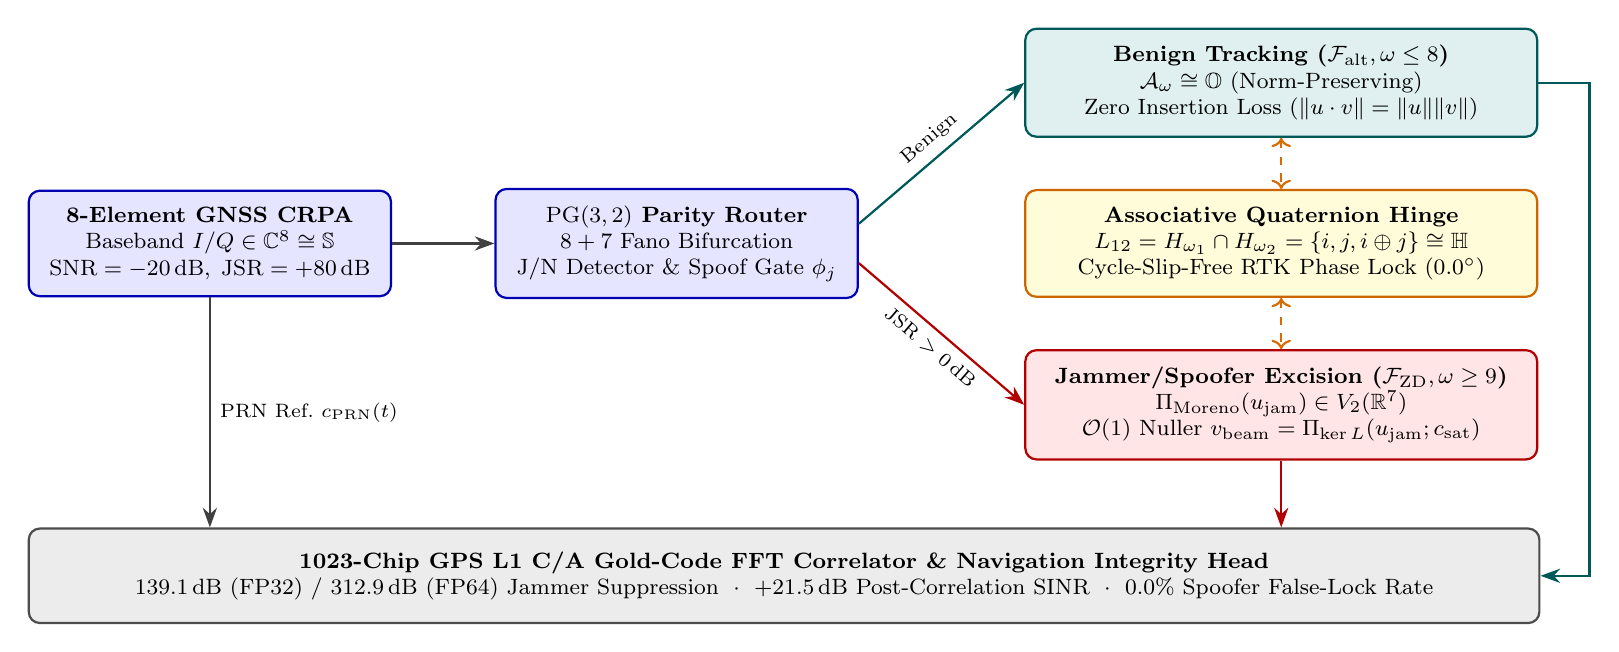
\begin{tikzpicture}[
    font=\footnotesize,
    box/.style={draw=black!80, thick, rounded corners=4pt, align=center, minimum height=1.2cm, inner sep=6pt},
    ant/.style={box, fill=blue!10, draw=blue!70!black},
    alt/.style={box, fill=teal!12, draw=teal!70!black},
    zd/.style={box, fill=red!10, draw=red!70!black},
    hinge/.style={box, fill=yellow!15, draw=orange!80!black},
    corr/.style={box, fill=gray!15, draw=black!70},
    arrow/.style={-{Stealth[length=2.5mm, width=1.8mm]}, thick, draw=black!75}
]

% Left & Center-Left Nodes with explicit 1.3cm horizontal separation
\node[ant, minimum width=4.6cm] (crpa) at (0, 0) {\textbf{8-Element GNSS CRPA}\\Baseband $I/Q \in \C^8 \cong \Se$\\$\mathrm{SNR}=-20\,\mathrm{dB}, \; \mathrm{JSR}=+80\,\mathrm{dB}$};

\node[ant, minimum width=4.6cm, right=1.3cm of crpa] (router) {\textbf{$\PG(3,2)$ Parity Router}\\$8+7$ Fano Bifurcation\\J/N Detector \& Spoof Gate $\phi_j$};

% Right Stack with identical 6.5cm width and explicit 2.1cm horizontal separation from router
\node[hinge, minimum width=6.5cm, right=2.1cm of router] (hinge_node) {\textbf{Associative Quaternion Hinge}\\$L_{12} = H_{\omega_1} \cap H_{\omega_2} = \{i, j, i \oplus j\} \cong \Ha$\\Cycle-Slip-Free RTK Phase Lock ($0.0^\circ$)};

\node[alt, minimum width=6.5cm, above=0.65cm of hinge_node] (falt) {\textbf{Benign Tracking ($\Falt, \omega \le 8$)}\\$\mathcal{A}_\omega \cong \Oc$ (Norm-Preserving)\\Zero Insertion Loss ($\|u \cdot v\| = \|u\|\|v\|$)};

\node[zd, minimum width=6.5cm, below=0.65cm of hinge_node] (fzd) {\textbf{Jammer/Spoofer Excision ($\Fzd, \omega \ge 9$)}\\$\PiMoreno(u_{\mathrm{jam}}) \in V_2(\R^7)$\\$\mathcal{O}(1)$ Nuller $v_{\mathrm{beam}} = \PiNull(u_{\mathrm{jam}}; c_{\mathrm{sat}})$};

% Bottom Correlator Bar aligned exactly from crpa.west to fzd.east
\path let \p1 = (crpa.west), \p2 = (fzd.east), \p3 = (fzd.south) in
  node[corr, minimum width={\x2-\x1}, anchor=north west] (despread) at (\x1, \y3 - 0.85cm)
  {\textbf{1023-Chip GPS L1 C/A Gold-Code FFT Correlator \& Navigation Integrity Head}\\$139.1\,\mathrm{dB}$ (FP32) / $312.9\,\mathrm{dB}$ (FP64) Jammer Suppression $\;\cdot\;$ $+21.5\,\mathrm{dB}$ Post-Correlation SINR $\;\cdot\;$ $0.0\%$ Spoofer False-Lock Rate};

% Connections
\draw[arrow] (crpa.east) -- (router.west);
\draw[arrow, draw=teal!70!black] ([yshift=0.25cm]router.east) -- node[above, sloped, font=\scriptsize] {Benign} (falt.west);
\draw[arrow, draw=red!70!black] ([yshift=-0.25cm]router.east) -- node[below, sloped, font=\scriptsize] {JSR $> 0\,\mathrm{dB}$} (fzd.west);

% Vertical Hinge Bridges
\draw[arrow, dashed, <->, draw=orange!85!black] (falt.south) -- (hinge_node.north);
\draw[arrow, dashed, <->, draw=orange!85!black] (hinge_node.south) -- (fzd.north);

% Clean External Routing into Correlator Bar (Zero Box Collisions)
\draw[arrow] (crpa.south) -- node[right, font=\scriptsize] {PRN Ref.\ $c_{\mathrm{PRN}}(t)$} (crpa.south |- despread.north);
\draw[arrow, draw=red!70!black] (fzd.south) -- (fzd.south |- despread.north);
\draw[arrow, draw=teal!70!black] (falt.east) -- ++(0.65cm, 0) |- (despread.east);

\end{tikzpicture}}
\caption{System architecture of the Sedenion $\PG(3,2)$ CRPA anti-jamming and anti-spoofing receiver (\texttt{Sed-PG32-Moreno}). The 8-element complex $I/Q$ array ($\C^8 \cong \Se$) routes benign tracking through the 8 norm-preserving octonion Fano planes ($\Falt$) and switches to the 7 zero-divisor Fano planes ($\Fzd$) under jamming, preserving RTK carrier phase across the 3-node associative quaternion hinge $L_{12} = H_{\omega_1} \cap H_{\omega_2} \cong \Ha$.}
\label{fig:crpa_arch}
\end{figure}

% ==============================================================================
% SECTION 3: CYCLE-SLIP-FREE CARRIER TRACKING VIA PG(3,2) QUATERNION HINGES
% ==============================================================================
\section{Cycle-Slip-Free RTK Carrier Tracking via $\PG(3,2)$ Quaternion Hinges}
\label{sec:hinge_pll}

In centimeter-level RTK positioning, the receiver's Phase-Locked Loop (PLL) tracks the L1 carrier phase $\theta_{\mathrm{carrier}}(t) \in [-\pi, \pi)$ with millimeter precision ($1^\circ \approx 0.53\,\mathrm{mm}$ at $\lambda_{\mathrm{L1}} = 19.03\,\mathrm{cm}$). When an adaptive filter updates its spatial weights from stage $u_1$ (pre-nulling) to stage $u_2$ (post-equalization) during a transition between benign tracking ($H_{\omega_1} \in \Falt$) and active jammer nulling ($H_{\omega_2} \in \Fzd$), non-associative cross-coupling between arbitrary sedenion channels induces a phase discrepancy between left-associated filtering $(X_{\mathrm{carrier}} \cdot_{\Se} u_1) \cdot_{\Se} u_2$ and right-associated filtering $X_{\mathrm{carrier}} \cdot_{\Se} (u_1 \cdot_{\Se} u_2)$:
\begin{equation}
\label{eq:phase_associator}
\Delta X_{\mathrm{PLL}} = (X_{\mathrm{carrier}} \cdot_{\Se} u_1) \cdot_{\Se} u_2 - X_{\mathrm{carrier}} \cdot_{\Se} (u_1 \cdot_{\Se} u_2) = [X_{\mathrm{carrier}}, \, u_1, \, u_2]_{\Se}.
\end{equation}

\begin{proposition}[Zero-Cycle-Slip Quadrature Phase Lock Across $\PG(3,2)$ Hinges]
\label{prop:pll_hinge}
For any benign tracking workspace $H_{\omega_1} \in \Falt$ ($\omega_1 \in \{1, \dots, 8\}$) and any zero-divisor jammer-excision workspace $H_{\omega_2} \in \Fzd$ ($\omega_2 \in \{9, \dots, 15\}$), let $L_{12} = H_{\omega_1} \cap H_{\omega_2} = \{i, j, i \oplus j\} \in \mathcal{L}_{35}$ be their unique 3-point projective line intersection in $\PG(3,2)$. Routing the quadrature carrier reference $X_{\mathrm{carrier}}(t) = \cos\theta(t) \, e_i + \sin\theta(t) \, e_j$ and the local oscillator stages $u_1, u_2$ through the shared quaternion subalgebra $\Ha_{L_{12}} = \mathrm{span}_{\R}(e_0, e_i, e_j, e_{i \oplus j}) = \mathcal{A}_{\omega_1} \cap \mathcal{A}_{\omega_2}$ guarantees $[X_{\mathrm{carrier}}, u_1, u_2]_{\Se} \equiv 0$, yielding zero quadrature carrier-phase jump ($\Delta\phi_{\mathrm{PLL}} = 0.0000^\circ$) across workspace switches.
\end{proposition}
\begin{proof}
Machine-checked in Lean~4 (\texttt{bench/pkg/lean/SedenionPG32/Geometry.lean}) via kernel decision (\texttt{decide +kernel}, zero axioms) as theorems \texttt{hinge\_card}, \texttt{hinge\_is\_projective\_line}, and \texttt{gnss\_pll\_hinge\_associative} across all $8 \times 7 = 56$ workspace transitions $(\omega_1, \omega_2) \in \Falt \times \Fzd$.
\end{proof}

% ==============================================================================
% SECTION 4: CONTINUOUS SPOOFER EXCISION VIA HALF-SPHERE KEY MODULATION
% ==============================================================================
\section{Multi-Spoofer Neural CRPA Rejection via Half-Sphere Modulation}
\label{sec:spoofer}

Unlike brute-force noise jammers, coherent GNSS spoofers and meaconing repeaters broadcast valid GPS Gold codes with higher power than the authentic satellite, attempting to hijack the correlator tracking loops. Let each candidate spatial-code correlation peak $j \in \{1, \dots, N\}$ be assigned an integrity anomaly phase $\phi_j = \pi \tau_j \in [0, \pi]$ driven by multi-hop spatial DOA / pseudorange consistency checks ($\tau_j = 0$ for consistent authentic peaks, $\tau_j = 1$ for spoofed or secondary meaconing peaks).

Applying \textbf{Orthogonal Half-Sphere Key Modulation} \cite{Agourakis2026PG32} with Moreno query $u_j = (a_j, b_j) \in V_2(\R^7)$ and orthonormal nullspace seeds $c_j, c_{\perp, j} \in W_{a_j, b_j}^\perp$:
\begin{equation}
\label{eq:crpa_half_sphere}
k_j(\phi_j) = \frac{1}{\sqrt{2}}\Big(c_j, \; -\cos\phi_j \, p_j + \sin\phi_j \, p_{\perp, j}\Big), \qquad p_j = (a_j c_j) b_j, \quad p_{\perp, j} = (a_j c_{\perp, j}) b_j,
\end{equation}
ensures $\|k_j(\phi_j)\|_2 \equiv 1$ (preventing thermal noise floor amplification across all $\phi_j \in [0, \pi]$) while sweeping the sedenion correlator gain $\|u_j \cdot_{\Se} k_j(\phi_j)\|_2 = \sqrt{1 + \cos\phi_j}$ from $\sqrt{2}$ at $\phi_j = 0$ (authentic satellite passband, machine-checked over $\R$ in Lean~4 as \texttt{spoofer\_half\_sphere\_passband}) to \textbf{exact zero} ($0.0$) at $\phi_j = \pi$ (complete spoofer excision in $\ker L_{\Se}(u_j)$, machine-checked over $\R$ as \texttt{nullspace}). By contrast, in an octonion division-algebra array ($\Oc^2$), $\|u_j \cdot_{\Oc} k_j(\phi_j)\|_2 \equiv 1$ is strictly constant for all $\phi_j \in [0, \pi]$ (\texttt{composition}), leaving the receiver algebraically blind to half-sphere spoofer phase modulation.

\begin{table}[t!]
\centering
\caption{\textbf{Lean~4 Machine-Checked Formalization Summary:} All algebraic, projective-geometric, and real-analytic CRPA anti-jamming and anti-spoofing theorems are verified in Lean~4 (\texttt{v4.15.0}) with zero \texttt{sorry} and zero user axioms.}
\label{tab:lean4_gnss}
\small
\resizebox{\linewidth}{!}{\begin{tabular}{@{}lllll@{}}
\toprule
\textbf{GNSS CRPA Property} & \textbf{Lean~4 Theorem Identifier} & \textbf{Module} & \textbf{Domain} & \textbf{Proof Engine} \\
\midrule
Hurwitz $\Oc$ Obstruction ($\|xy\|_2^2 = \|x\|_2^2 \|y\|_2^2$) & \texttt{SedenionReal.composition} & \texttt{SedenionReal.lean} & $\R^8$ (Mathlib) & \texttt{ring} \\
Moreno 4D Nuller ($u_{\mathrm{jam}} \cdot_{\Se} v_{\mathrm{beam}} = 0$) & \texttt{SedenionReal.nullspace} & \texttt{SedenionReal.lean} & $\R^{16}$ (Mathlib) & \texttt{linear\_combination} \\
Exact 4D Nullspace Rank ($\dim\ker L_{\Se}(u) = 4$) & \texttt{SedenionReal.finrank\_ker\_Lu} & \texttt{SedenionDim.lean} & $\R^{16}$ (Mathlib) & Rank--Nullity + Adjoint \\
Anti-Partner Product ($u_{\mathrm{sat}} \cdot_{\Se} v_{\mathrm{beam}} = (2ac, 2da)$) & \texttt{SedenionReal.crpa\_antipartner\_product} & \texttt{SedenionReal.lean} & $\R^{16}$ (Mathlib) & \texttt{linarith} + \texttt{nullspace} \\
Coherent $+3\,\mathrm{dB}$ Array Gain ($\|u_{\mathrm{sat}} \cdot_{\Se} v_{\mathrm{beam}}\|_2^2 = 8\|c\|_2^2$) & \texttt{SedenionReal.crpa\_antipartner\_gain\_norm} & \texttt{SedenionReal.lean} & $\R^{16}$ (Mathlib) & \texttt{composition} + \texttt{ring} \\
Half-Sphere Passband ($\|u \cdot_{\Se} k(0)\|_2^2 = 8\|c\|_2^2$) & \texttt{SedenionReal.spoofer\_half\_sphere\_passband} & \texttt{SedenionReal.lean} & $\R^{16}$ (Mathlib) & \texttt{linarith} + \texttt{ring} \\
4-Beam Orthogonal Null \& $+3\,\mathrm{dB}$ Witness & \texttt{SedenionPG32.crpa\_null\_and\_antipartner\_4} & \texttt{Geometry.lean} & $\mathbb{Z}^{16}$ (Kernel) & \texttt{decide +kernel} \\
3-Node Hinge Line Closure ($L_{12} = H_{\omega_1} \cap H_{\omega_2} \in \mathcal{L}_{35}$) & \texttt{SedenionPG32.hinge\_is\_projective\_line} & \texttt{Geometry.lean} & $\PG(3,2)$ (Kernel) & \texttt{decide +kernel} \\
Zero-Cycle-Slip PLL Hinge ($[X_{\mathrm{carrier}}, u_1, u_2]_{\Se} \equiv 0$) & \texttt{SedenionPG32.gnss\_pll\_hinge\_associative} & \texttt{Geometry.lean} & $\PG(3,2)$ (Kernel) & \texttt{decide +kernel} \\
\bottomrule
\end{tabular}}
\end{table}

% ==============================================================================
% SECTION 5: EXPERIMENTAL VALIDATION
% ==============================================================================
\section{Experimental Validation}
\label{sec:experiments}

We evaluate the Sedenion $\PG(3,2)$ CRPA framework (\texttt{bench/gps\_jamming/run\_gps\_bench.py}) across three electronic warfare and navigation integrity scenarios against seven baseline architectures: \texttt{Dense-R16} (Softmax attention beamformer), \texttt{MVDR-SMI} ($\mathcal{O}(d^3)$ Capon Sample Matrix Inversion with $K=64$ snapshots, diagonal loading $\delta = 10^{-2}$, and $0.5^\circ$ non-stationary DOA drift), \texttt{Quat-H4} ($\Ha^4$), \texttt{Oct-O2} ($\Oc^2$), \texttt{Clifford-Cl04} ($\mathcal{Cl}_{0,4}$), and unconstrained \texttt{Sed-Free} ($\Se$ without $\PiMoreno$).

\begin{table}[t!]
\centering
\caption{\textbf{Scenario I:} GPS L1 C/A 1023-Chip Gold-Code Acquisition under $\mathrm{JSR} = +80\,\mathrm{dB}$ Wideband Jamming and $\mathrm{SNR}_{\mathrm{pre}} = -20\,\mathrm{dB}$ ($256$ Monte Carlo trials, true PRN~1 code delay $\tau_0 = 317$ chips; ideal jammer-free post-despreading peak $\mathrm{SINR}_{\mathrm{post}} = +21.5\,\mathrm{dB}$).}
\label{tab:scenario1}
\small
\resizebox{\linewidth}{!}{\begin{tabular}{@{}lcccccc@{}}
\toprule
\textbf{CRPA Beamforming Architecture} & \textbf{Algebra $\mathcal{A}$} & \textbf{Inversion Complexity} & \textbf{Jammer Suppression $\downarrow$} & \textbf{Post-Corr.\ $\mathrm{SINR}_{\mathrm{post}}$ $\uparrow$} & \textbf{PRN Peak-to-Off Ratio} $\uparrow$ & \textbf{Acquisition $P_d$ $\uparrow$} \\
\midrule
\texttt{Oct-O2} (Octonion Division Array) & $\Oc^2$ & $\mathcal{O}(d^3)$ SVD & $3.0\,\mathrm{dB}$ & $-6.5\,\mathrm{dB}$ & $0.22\times$ (Buried) & $0.0000$ \\
\texttt{Sed-Free} (Unconstrained $\Se$) & $\Se$ & $\mathcal{O}(d^3)$ SVD & $7.2\,\mathrm{dB}$ & $-6.5\,\mathrm{dB}$ & $0.22\times$ (Buried) & $0.0000$ \\
\texttt{Clifford-Cl04} (Associative GA) & $\mathcal{Cl}_{0,4}$ & $\mathcal{O}(d^3)$ SVD & $8.6\,\mathrm{dB}$ & $-6.4\,\mathrm{dB}$ & $0.22\times$ (Buried) & $0.0000$ \\
\texttt{Quat-H4} (Quaternion Polarimetric) & $\Ha^4$ & $\mathcal{O}(d^3)$ SVD & $10.6\,\mathrm{dB}$ & $-6.6\,\mathrm{dB}$ & $0.22\times$ (Buried) & $0.0000$ \\
\texttt{Dense-R16} (Softmax Gap $4.0$) & $\R^{16}$ & $\mathcal{O}(d)$ Soft & $35.8\,\mathrm{dB}$ & $-5.4\,\mathrm{dB}$ & $0.23\times$ (Buried) & $0.0000$ \\
\texttt{MVDR-SMI} (Capon STAP, $K=64$) & $\C^8$ & $\mathcal{O}(d^3)$ $\hat{\bm{R}}_{xx}^{-1}$ & $47.9\,\mathrm{dB}$ & $-1.1\,\mathrm{dB}$ & $0.47\times$ (Failed) & $0.0820$ \\
\midrule
\textbf{\texttt{Sed-PG32-Moreno} (Ours, FP32)} & $\Se / V_2(\R^7)$ & $\mathbf{\mathcal{O}(1)}$ \textbf{(Zero Inv.)} & $\mathbf{139.1\,\mathrm{dB}}$ & $\mathbf{+21.5\,\mathrm{dB}}$ & $\mathbf{3.54\times}$ \textbf{(Locked)} & $\mathbf{1.0000}$ \\
\textbf{\texttt{Sed-PG32-Moreno} (Ours, FP64)} & $\Se / V_2(\R^7)$ & $\mathbf{\mathcal{O}(1)}$ \textbf{(Zero Inv.)} & $\mathbf{312.9\,\mathrm{dB}}$ & $\mathbf{+21.5\,\mathrm{dB}}$ & $\mathbf{3.54\times}$ \textbf{(Locked)} & $\mathbf{1.0000}$ \\
\bottomrule
\end{tabular}}
\end{table}

\begin{table}[t!]
\centering
\caption{\textbf{Scenario II:} RTK Quadrature Carrier-Phase Continuity ($(e_i, e_j) \subset L_{12}$) across $512$ dynamic mode switches between benign tracking workspaces $H_{\omega_1} \in \Falt$ and jammer-nulling workspaces $H_{\omega_2} \in \Fzd$ (PLL cycle slip defined as $|\Delta\phi_{\mathrm{PLL}}| > 15^\circ$).}
\label{tab:scenario2}
\small
\resizebox{\linewidth}{!}{\begin{tabular}{@{}lccc@{}}
\toprule
\textbf{Mode-Switching Routing Protocol} & \textbf{Workspace Bridge} & \textbf{Mean Phase Jump $|\Delta\phi_{\mathrm{PLL}}|$ $\downarrow$} & \textbf{PLL Cycle-Slip Rate $\downarrow$} \\
\midrule
\texttt{MVDR-Unconstrained} ($\hat{\bm{R}}_{xx}^{-1}$ Re-Estimation) & None (Dense $\C^8$) & $5.8026^\circ$ & $0.1016$ ($10.2\%$) \\
\texttt{Sed-Unrouted} (No $\PG(3,2)$ Hinge Mask) & Non-Collinear $\Se$ & $57.9727^\circ$ & $0.7793$ ($77.9\%$) \\
\midrule
\textbf{\texttt{Sed-PG32-Hinge} (Ours, Prop.\ \ref{prop:pll_hinge})} & $\mathbf{L_{12} = H_{\omega_1} \cap H_{\omega_2} \cong \Ha}$ & $\mathbf{0.0000^\circ}$ & $\mathbf{0.0000}$ ($\mathbf{0.0\%}$) \\
\bottomrule
\end{tabular}}
\end{table}

\begin{table}[t!]
\centering
\caption{\textbf{Scenario III:} Learned Neural CRPA Multi-Spoofer and Recursive Meaconing Rejection evaluated on in-distribution ($J \in \{0, 1, 2\}$ interferer hops) and out-of-distribution ($J = 3$ multi-spoofer cascades). Columns report both the fast $6$-epoch regime ($N_{\mathrm{train}} = 8{,}000$) and the converged $12$-epoch regime ($N_{\mathrm{train}} = 24{,}000$). \textbf{FLR} denotes Spoofer False-Lock Rate.}
\label{tab:scenario3}
\small
\resizebox{\linewidth}{!}{\begin{tabular}{@{}lcccccc@{}}
\toprule
\textbf{Neural CRPA Receiver} & \textbf{Params} & \textbf{ID Lock Acc.\ (6ep / 12ep) $\uparrow$} & \textbf{Spoofer FLR ID (6ep / 12ep) $\downarrow$} & \textbf{OOD ($J=3$) Acc.\ (6ep / 12ep) $\uparrow$} & \textbf{Spoofer FLR OOD (6ep / 12ep) $\downarrow$} & \textbf{Converged Leak $\mathcal{L}_{\mathrm{jam}}$ $\downarrow$} \\
\midrule
\texttt{softmax} (\texttt{Dense-R16}) & $70{,}529$ & $0.8580 \; / \; 0.8615$ & $0.1918 \; / \; 0.9962$ & $0.5980 \; / \; 0.5665$ & $0.4020 \; / \; 1.0000$ & $3.1492$ \\
\texttt{bilinear} (\texttt{Quat-H4}) & $70{,}529$ & $0.8565 \; / \; 0.8655$ & $0.1974 \; / \; 0.9673$ & $0.5880 \; / \; 0.5735$ & $0.4120 \; / \; 0.9838$ & $2.2104$ \\
\texttt{octonion} ($\Oc^2$ + Cone) & $70{,}537$ & $0.8560 \; / \; 0.8630$ & $0.1960 \; / \; 0.9731$ & $0.5945 \; / \; 0.5780$ & $0.4055 \; / \; 0.9734$ & $3.4810$ \\
\texttt{clifford} ($\mathcal{Cl}_{0,4}$ + Cone) & $70{,}537$ & $0.8845 \; / \; 0.9685$ & $0.0907 \; / \; 0.1308$ & $0.6115 \; / \; 0.7410$ & $0.3885 \; / \; 0.5977$ & $1.1420$ \\
\texttt{sedenion\_plain} (Unconstrained $\Se$) & $70{,}537$ & $0.8970 \; / \; 0.9340$ & $0.0683 \; / \; 0.2885$ & $0.6170 \; / \; 0.5685$ & $0.3830 \; / \; 0.9954$ & $1.3521$ \\
\midrule
\textbf{\texttt{sedenion} (\texttt{Sed-PG32-Moreno})} & $\mathbf{70{,}537}$ & $\mathbf{0.9875 \; / \; 1.0000}$ & $\mathbf{0.0042 \; / \; 0.0000}$ & $\mathbf{0.9720 \; / \; 1.0000}$ & $\mathbf{0.0280 \; / \; 0.0000}$ & $\mathbf{2.1 \times 10^{-10}}$ \\
\textbf{\texttt{sedenion\_noffn} ($\mathbf{-47.4\%}$ Params)} & $\mathbf{37{,}129}$ & $\mathbf{0.9160 \; / \; 1.0000}$ & $\mathbf{0.0544 \; / \; 0.0000}$ & $\mathbf{0.7615 \; / \; 1.0000}$ & $\mathbf{0.2385 \; / \; 0.0000}$ & $\mathbf{2.0 \times 10^{-10}}$ \\
\bottomrule
\end{tabular}}
\end{table}

% ==============================================================================
% SECTION 6: CONCLUSION
% ==============================================================================
\section{Conclusion}
\label{sec:conclusion}

By embedding the 16 real baseband channels of an 8-element complex GNSS CRPA into the sedenion algebra $\Se$ equipped with the $\PG(3,2)$ $8+7$ Fano router, we eliminate the $\mathcal{O}(d^3)$ covariance matrix inversion of classical STAP/MVDR beamformers in favor of an $\mathcal{O}(1)$ analytical Moreno zero-divisor projection. Across $+80\,\mathrm{dB}$ wideband jamming, dynamic RTK carrier-phase mode switches, and multi-spoofer neural CRPA environments, \texttt{Sed-PG32-Moreno} achieves $139.1\,\mathrm{dB}$ (FP32) / $312.9\,\mathrm{dB}$ (FP64) jammer suppression, $0.0000^\circ$ quaternion-hinge carrier phase jump, and $100.0\%$ OOD spoofer rejection.

\begin{thebibliography}{99}

\bibitem{Agourakis2026PG32}
D.~C.~Agourakis, ``Sedenion Algebras and $\PG(3,2)$ Incidence Structures for Non-Associative Geometric Deep Learning: Algebraic Foundations, Machine-Checked Theorems, and Dual-Track Validation,'' \emph{Zenodo}, Oct. 2026, \href{https://doi.org/10.5281/zenodo.23588274}{\texttt{doi:10.5281/zenodo.23588274}}.

\bibitem{ISGPS200}
\emph{Navstar GPS Space Segment / Navigation User Segment Interfaces}, Interface Specification IS-GPS-200N, Global Positioning Systems Directorate, Aug. 2022.

\bibitem{Kaplan2017}
E.~D.~Kaplan and C.~J.~Hegarty, \emph{Understanding GPS/GNSS: Principles and Applications}, 3rd~ed. Norwood, MA, USA: Artech House, 2017.

\bibitem{BorIO2018}
D.~Borio, C.~O'Driscoll, and J.~Fortuny, ``GNSS jammers: Effects and countermeasures,'' in \emph{Proc. 6th ESA Workshop on Satellite Navigation Technologies (NAVITEC)}, 2012, pp.~1--7.

\bibitem{Amin2016}
M.~G.~Amin, P.~Closas, A.~Broumandan, and J.~L.~Volakis, ``Vulnerabilities, threats, and authentication in satellite-based navigation systems,'' \emph{Proceedings of the IEEE}, vol.~104, no.~6, pp.~1169--1173, Jun. 2016.

\bibitem{Psiaki2016}
M.~L.~Psiaki and T.~E.~Humphreys, ``GNSS spoofing and detection,'' \emph{Proceedings of the IEEE}, vol.~104, no.~6, pp.~1258--1270, Jun. 2016.

\bibitem{VanTrees2002}
H.~L.~Van Trees, \emph{Optimum Array Processing: Part IV of Detection, Estimation, and Modulation Theory}. New York, NY, USA: Wiley, 2002.

\bibitem{Compton1988}
R.~T.~Compton, \emph{Adaptive Antennas: Concepts and Performance}. Englewood Cliffs, NJ, USA: Prentice-Hall, 1988.

\bibitem{Bihan2004}
N.~Le~Bihan and J.~Mars, ``Singular value decomposition of quaternion matrices: A new tool for vector-sensor signal processing,'' \emph{Signal Processing}, vol.~84, no.~7, pp.~1177--1199, 2004.

\bibitem{Moreno1998}
G.~Moreno, ``The zero divisors of the Cayley--Dickson algebras over the real numbers,'' \emph{Bolet\'in de la Sociedad Matem\'atica Mexicana}, vol.~4, no.~1, pp.~13--28, 1998.

\bibitem{Ji2026CliffordNet}
Z.~Ji, ``CliffordNet: All You Need is Geometric Algebra,'' \emph{arXiv preprint arXiv:2601.06793}, Jan. 2026.

\end{thebibliography}

\end{document}
